\section{Les arbres et grilles d'arbres}

\subsection{Les arbres binaires}
\paragraph{Diamètre d'un arbre binaire : } Un arbre est constitué d'un ensemble de niveaux, le niveau 0 étant occupé par la racine de l'arbre.
Les niveaux se répartissent donc de 0 à $p$ où $p$ est par définition la hauteur ou la profondeur de l'arbre. Chaque niveau $i$ est occupé 
par $k^{i}$  nœuds dans un arbre $k$-naire, par $2^{i}$ pour un arbre binaire. 
Par conséquent, à la profondeur $p$, un arbre binaire complet aura donc $f = 2^{p}$ 
feuilles. Un arbre binaire complet sera constitué de $2^{p+1}-1 = 2f-1$ nœuds y compris les feuilles.
La plus grande distance entre deux nœuds, i.e. le diamètre de l'arbre, est donc le nombre d'arêtes 
du chemin passant par la racine et joignant deux feuilles. Ce qui donne : \[D = 2p = 2\log_2(f)\]


puisque la profondeur est liée au nombre de feuilles par \[p = \log_2(f)\]

% $a_{n}^{m}$

\paragraph{Bissection d'un arbre binaire : } La bissection est le nombre minimal d'arêtes à supprimer pour qu'un graphe initialement
connexe se sépare en deux composantes connexes possédant le même nombre de nœuds à une unité près.
Pour un arbre binaire, ce nombre minimal est obtenu en supprimant une des deux arêtes liées à la racine. On trouve
donc dans ce cas une bissection égale à 1.

\begin{figure}[htp]
  \centering
  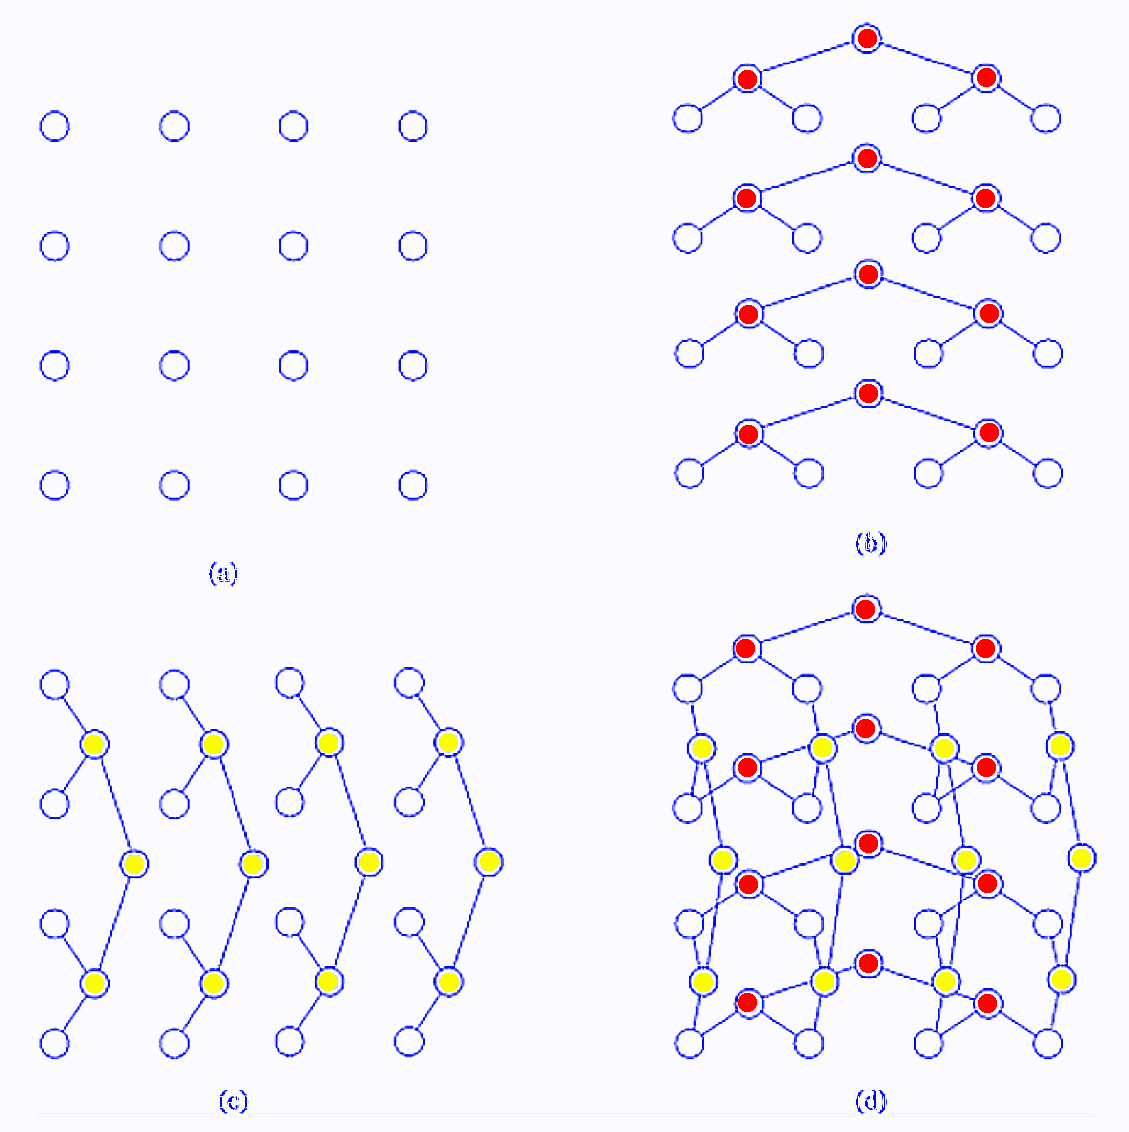
\includegraphics[width=10cm]{images/gda}
  \caption{Grille d'arbre 2-D construite sur une grille $N \times N$ avec $N = 4$ (a) à laquelle on connecte 4 arbres binaires horizontaux (b) et 
  4 arbres binaires verticaux (c) pour obtenir la grille d'arbres (d).}
  \label{fig:gda}
\end{figure}
\subsection{Les grilles d'arbres}

\paragraph{Définition d'une grille d'arbres bidimensionnelle :}
Une grille d'arbre bidimensionnelle, \textit{mesh of trees} en anglais ou MOT en abrégé, est construite à partir d'une grille
bidimensionnelle reliée par des arbres binaires, verticalement et horizontalement comme illustré figure \ref{fig:gda}.
Les nœuds de la grille constituent les feuilles des arbres. On a donc $2N$ arbres de profondeur $p = \log_2(N)$.
Chacun des $2N$ arbres est composé de $(N-1)$ nœuds internes et de $N$ feuilles. On a donc un nombre total de nœuds dans la grille
d'arbres égal à la somme des nœuds de la grille $N \times N$, soit $N^2$ et du nombre de nœuds ajoutés par les arbres, soit $2N(N-1)$. 
Une grille d'arbres $N\times N$ est donc composée de $3N^2 - 2N$ nœuds. On montre enfin qu'une grille d'arbres comporte $2N(2^{p+1}-2) = 4N^2-4N$ arêtes.



\paragraph{Diamètre d'une grille d'arbres : } Le diamètre est la distance ``diagonale'' entre le nœud supérieur gauche et inférieur droit. La géométrie
carrée implique que cette distance est le double de la distance qui sépare le nœud supérieur gauche et le nœud inférieur gauche. Or ces 2
nœuds sont les feuilles d'un arbre binaire qui compte $N$ feuilles dont le diamètre est $D = 2p = 2\log_2(N)$. Le diamètre d'une grille d'arbres
est donc : \[D' = 4\log_2(N)\] 

\paragraph{Bissection d'une grille d'arbres : } La figure \ref{fig:gda} (c) montre qu'en déconnectant les $N = 4$ racines des arbres verticaux, 
on aboutit à deux sous-réseaux de même taille si on affecte une fois sur deux les nœuds racines ainsi déconnectés au
sous-réseau supérieur puis au sous réseau inférieur. La bissection est donc $N$.

\paragraph{Bilan : } Les grilles d'arbres sont des architectures performantes car elles jouissent à la fois d'un diamètre faible, donc de connexions 
plus rapides et directes, d'un degré constant (1, 2 ou 3) et d'un nombre d'arêtes modéré, ce qui les rendent particulièrement évolutives. Le bissection, que l'on peut définir par rapport à la connectivité entre deux parties de la structure et la maîtrise du risque lié aux "goulots d'étranglement", n'est pas la plus élevée mais reste acceptable (voir 4.1 Comparaison des différentes architectures), et bien supérieure à celle d'un arbre binaire classique.


\subsection{Implémentation du produit matrice-vecteur sur une grille d'arbres : }

On suppose qu'on dispose d'une grille d'arbres $N \times N$ sur laquelle on cherche à effectuer le produit matrice-vecteur $Y = AX$ où $A = (a_{ij})$, $X = (x_i)$
et $Y=y_j$ avec $0\leq i,j\leq N-1$. 


\begin{enumerate}
 \item On introduit $x_i$ par la racine de l'arbre horizontal $i$ non représenté sur la figure \ref{fig:gda2}(b), $0\leq i\leq N-1$. 
 \item Les $x_i$ sont transmis aux feuilles au travers des arbres horizontaux de telle 
 sorte que chaque feuille de l'arbre de la ligne $i$ 
 reçoit $x_i$ à l'étape $\log N$.
 \item On introduit $(a_{ij})$ dans la feuille $(i,j)$ via les entrées $I_i$ à l'étape $\log N$. 
 \item La feuille $(i,j)$ peut alors calculer le produit $a_{ij}x_j$.
 \item Les résultats sont sommés vers la racine des arbres verticaux.
\end{enumerate}



\begin{figure}[htp]
  \centering
  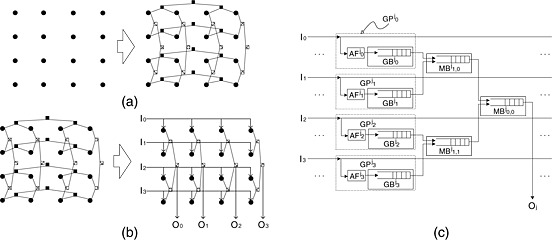
\includegraphics[width=15cm]{images/gda2}
  \caption{Grille d'arbres pour illustrer le principe du calcul d'un produit matrice-vecteur.}
  \label{fig:gda2}
\end{figure}


Après $2\log N$ étapes, la valeur \[y_i = \sum_{j=1}^{N} a_{ij}x_j\] est disponible dans 
la racine de la $i^{e}$ colonne désignée par $O_i$ sur la figure \ref{fig:gda2} (b). 
